%%
%% Kapitel:
%%
%%======================================================================

\section{Bilder JPG-format}
\label{sec:BilderJGP}
%
Mit \emph{JPG} muss weniger getrickst werden  als mit eps.
Allerdings hat YAP, der Viewer f�r dvi-Dateien manchmal Probleme.
%
%
\subsection{Erzeugung}
%
Wie k�nnen jpg-Dateien aus �blichen Anwendungen heraus erzeugt werden?

Beispielsweise ist Folgendes m�glich:
\begin{enumerate}
	\item Diagramm mit Excel erzeugen, 
	\item markieren, kopieren,
	\item in MS-PAINT einf�gen,
	\item als png- und/oder jpg-Datei speichern
	\item oder in pdf-Datei drucken.
\end{enumerate}
png-Dateien sind auch f�r dvi-Formate geeignet und in der Qualit�t h�ufig besser als jpg.


Vorzugsweise sollten keine absoluten Einheiten f�r die Bildgr��e verwendet werden.
Beim Umformatieren k�nnte es sonst dazu kommen, dass das Bild nicht 
mehr an die Stelle passt. Darum lieber mit einem Teil von {\verb#\textwidth#}
die Bildbreite angeben (\zB {\verb#0.7\textwidth#}).
%
{\begin{figure}[htb]
              \begin{center}
              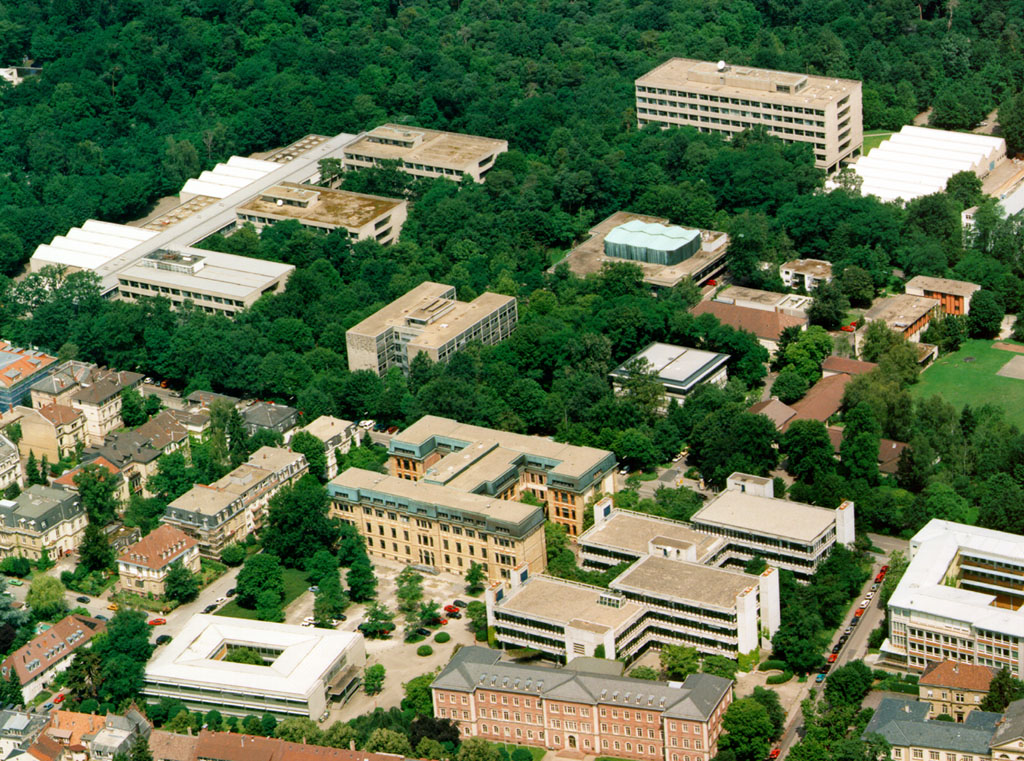
\includegraphics[width=0.5\textwidth]{060_Bilder/luftbild.jpg}
              \caption
              [Text des Luftbilds f�r das Abbildungsverzeichnis]              
              {\label{fig:bildJPEG}%
              Bild als JPEG}%
              \end{center}
              \end{figure}
             }

\fg{tbh}{060_Bilder/luftbild.jpg}{0.5\textwidth}{0}
        {Gleiches Bild mit Makro}
        {Gleiches Bild mit Makro gezeigt}

\fgB{060_Bilder/Kerbschlag.jpg}{!h}{0.6\textwidth}{0}%
    {Au�en: Eine l�ngere Bildunterschrift, die auch �ber mehrere Zeilen gehen kann}%
    {o}{Beside outer}

\fgB{060_Bilder/Kerbschlag.jpg}{!h}{0.4\textwidth}{0}%
    {Innen: Eine l�ngere Bildunterschrift, die auch �ber mehrere Zeilen gehen kann}%
    {i}{Beside inner}


\begin{figure}[]
              \begin{center}
              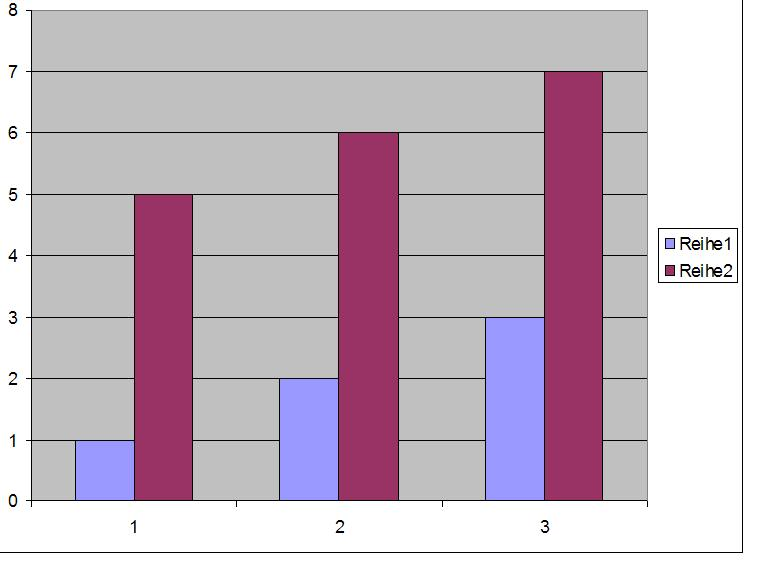
\includegraphics[width=0.8\textwidth]{060_Bilder/Excel-Paint.png}
              \caption%
              [Excel - Paint (copy and paste) save png]              
              {
              \label{fig:excelPaintpng}%
              Excel-Paint png
              }%
              \end{center}
              \end{figure}

\begin{figure}[]
              \begin{center}
              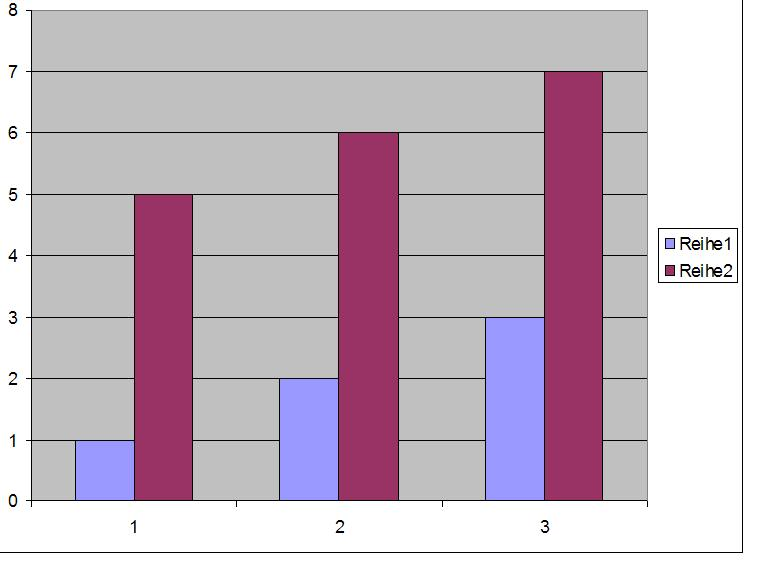
\includegraphics[width=0.8\textwidth]{060_Bilder/Excel-Paint.jpg}
              \caption
              [Excel - Paint (copy and paste) save jpg ]              
              {\label{fig:excelPaintjpg}%
              Excel-Paint jpg}%
              \end{center}
              \end{figure}

\begin{figure}[]
              \begin{center}
              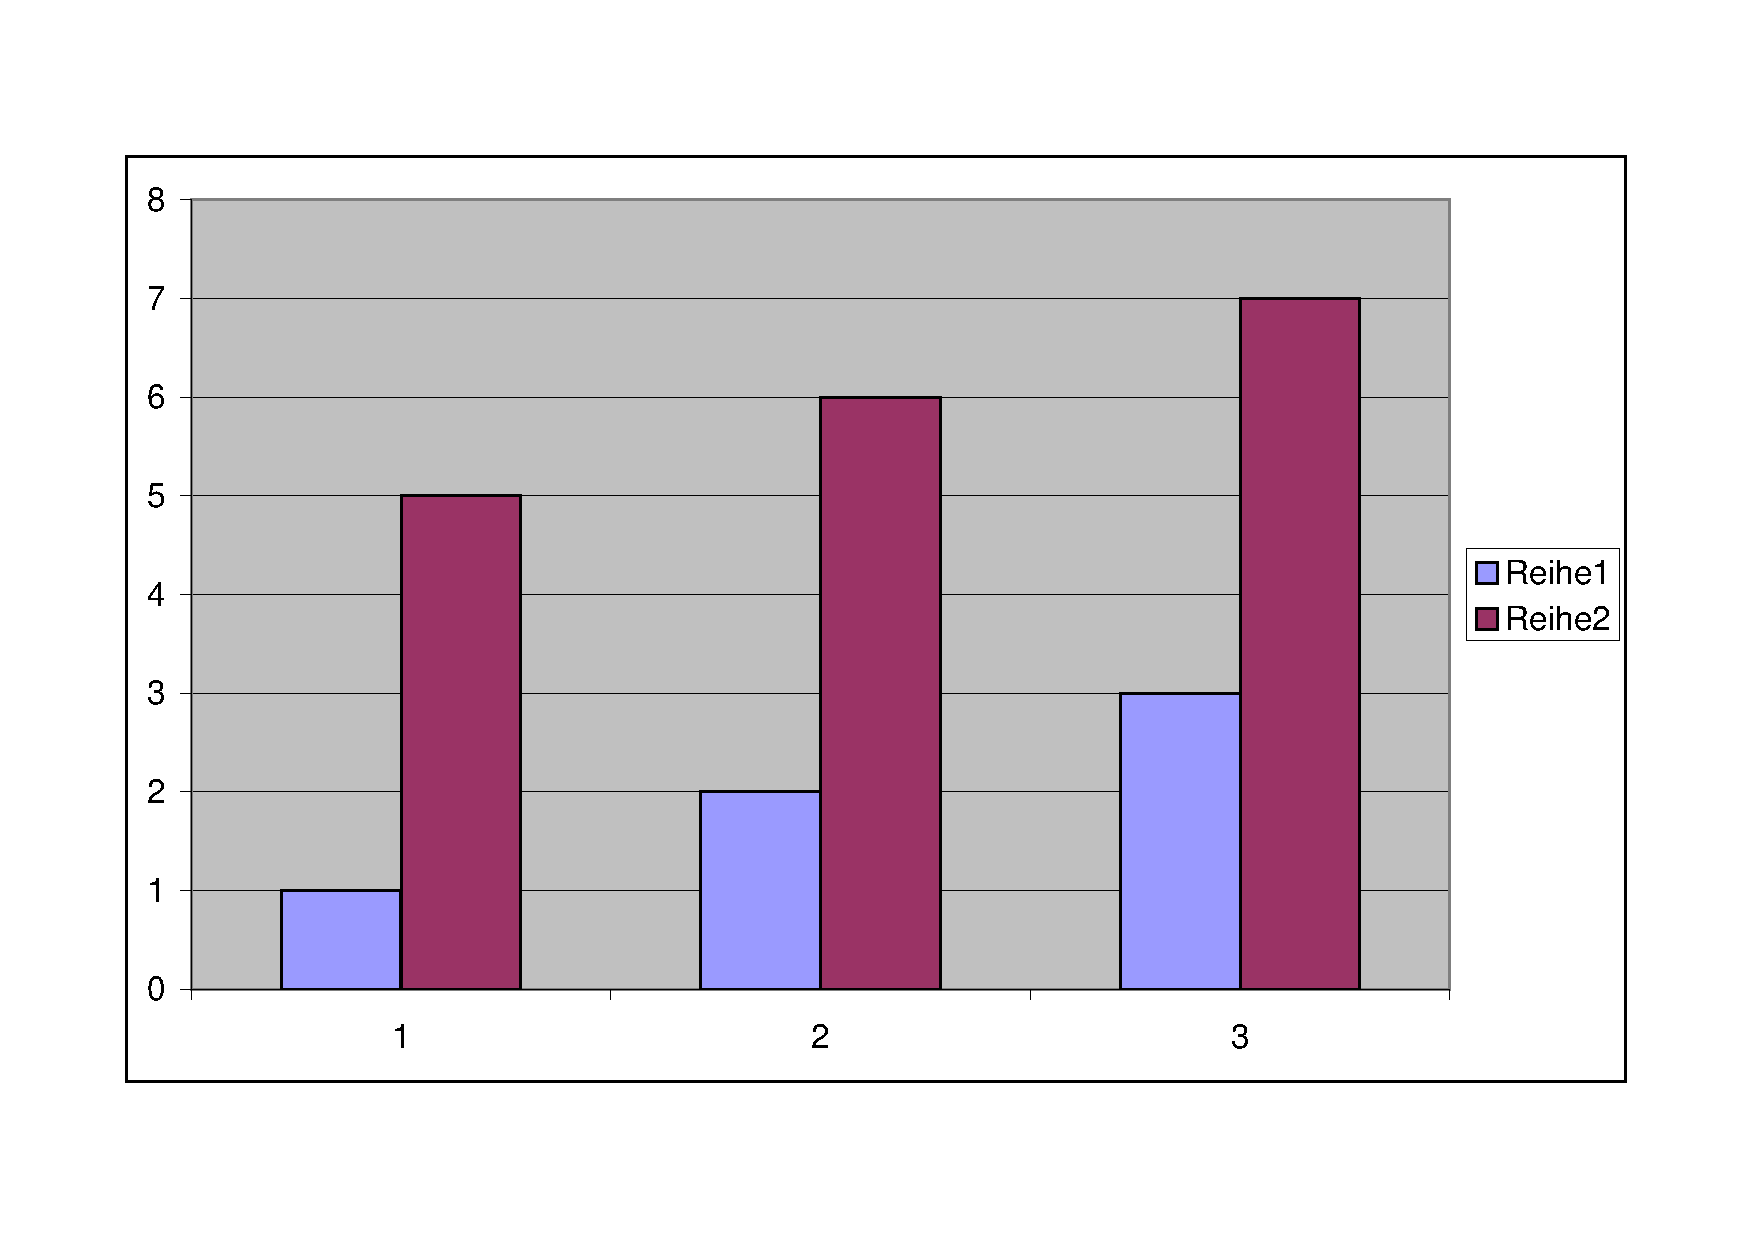
\includegraphics[width=0.8\textwidth]{060_Bilder/Excel-druck.pdf}
              \caption
              [Excel Druck pdf im AbbVerZeich]              
              {
              \label{fig:excelpdf}%
              Unterschrift Excel Druck pdf
              }%
              \end{center}
              \end{figure}
%                         
\clearpage
%